\section{驱动盒三维模型构建}
\begin{procedure}
\item 切换三维视图方向

为方便观察三维模型的构建,将AutoCAD的视图方向切换为西南等轴测。
\begin{lstlisting}
命令: -VIEW
输入选项 [?/删除(D)/正交(O)/恢复(R)/保存(S)/设置(E)/窗口(W)]: swiso
\end{lstlisting}

由于圆柱体的特征圆位于主视图,因此我们使用UCS命令将用户坐标的$z$位置修改为垂直于主视图方向。

\begin{lstlisting}
命令:  UCS
当前 UCS 名称: *世界*
指定 UCS 的原点或 [面(F)/命名(NA)/对象(OB)/上一个(P)/视图(V)/世界(W)/X/Y/Z/Z 轴(ZA)] <世界>: za
指定新原点或 [对象(O)] <0,0,0>:
在正 Z 轴范围上指定点 <0.0000,0.0000,1.0000>: 0,1,0
\end{lstlisting}

\begin{figure}[htbp]
\centering
\begin{floatrow}[2]
\ffigbox{\caption{$\phi 36$圆柱体}\label{fig:qudonghejianmo1}}{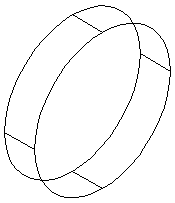
\includegraphics[width=0.4\columnwidth]{qudonghejianmo1}}
\ffigbox{\caption{制作倒角边}\label{fig:qudonghejianmo2}}{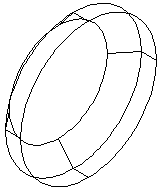
\includegraphics[width=0.4\columnwidth]{qudonghejianmo2}}
\end{floatrow}
\end{figure}

\item 构建$\phi 36$圆柱体

首先,运用圆柱体命令来构建$\phi 36$圆柱体,在AutoCAD的绘图区内任意选择一点作为圆柱体的圆心。绘图结果如图\ref{fig:qudonghejianmo1} 所示。

\begin{lstlisting}
命令: CYLINDER
指定底面的中心点或 [三点(3P)/两点(2P)/切点、切点、半径(T)/椭圆(E)]:
指定底面半径或 [直径(D)]: 18
指定高度或 [两点(2P)/轴端点(A)]: 8
\end{lstlisting}

\item 构建$\phi 36$圆柱体倒角边

接下来,构建$\phi 36$圆柱体倒角边,结果如图\ref{fig:qudonghejianmo2}
\begin{lstlisting}
命令: CHAMFEREDGE
距离 1 = 1.0000,距离 2 = 1.0000
选择一条边或 [环(L)/距离(D)]: d
指定距离 1 或 [表达式(E)] <1.0000>: 5
指定距离 2 或 [表达式(E)] <1.0000>: 4
选择一条边或 [环(L)/距离(D)]:
选择同一个面上的其他边或 [环(L)/距离(D)]:
按 Enter 键接受倒角或 [距离(D)]:
\end{lstlisting}

\item 拉伸面构建圆柱体


由于$\phi 36$圆柱体后面的圆柱体的直径并没有直接绘出,而是利用与$\phi 36$ 圆柱体之间的关系来间接获得,其直径与$\phi 36$ 圆柱体倒角边后所形成的圆的直径是一致的,因此采用拉伸面来完成该圆柱体的构建是最方便的方法。为方便选择拉伸平面,需要先将视图方向切换为东北等轴测。

\begin{lstlisting}
命令: -view 
输入选项 [?/删除(D)/正交(O)/恢复(R)/保存(S)/设置(E)/窗口(W)]: neiso
\end{lstlisting}

\yaodian{适当的等轴测视三维视图方向能够有利于三维模型边或者面的选择。}

要完成拉伸面的操作,需要AutoCAD中调用拉伸面命令,其方法有:
\begin{itemize}
	\item 键盘输入solidedit\index{solidedit,实体编辑}并选择【面(F)】选项中的【拉伸(E)】选项
	\item 【修改】$\rightarrow$【实体编辑】$\rightarrow$【面拉伸】
	\item 【实体编辑】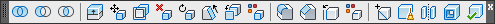
\includegraphics[scale=0.45]{solidedittools.png}工具中的
\includegraphics[scale=0.45]{faceextude.png}图标	
\end{itemize}

调用拉伸面命令后会出现下面的命令提示。

\begin{lstlisting}
命令: solidedit
实体编辑自动检查:  SOLIDCHECK=1
输入实体编辑选项 [面(F)/边(E)/体(B)/放弃(U)/退出(X)] <退出>: f
输入面编辑选项
[拉伸(E)/移动(M)/旋转(R)/偏移(O)/倾斜(T)/删除(D)/复制(C)/颜色(L)/材质(A)/放弃(U)/退出(X)] <退出>: e
\end{lstlisting}

\begin{figure}[htbp]
\centering
\subfloat[]{\label{fig:qudonghejianmo3}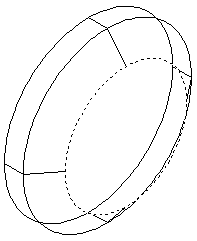
\includegraphics[width=0.2\columnwidth]{qudonghejianmo3}}\hspace{60pt}
\subfloat[]{\label{fig:qudonghejianmo4}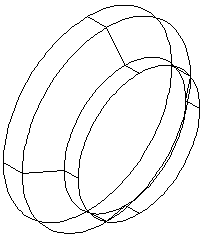
\includegraphics[width=0.2\columnwidth]{qudonghejianmo4}}
\caption{拉伸面操作}%
\end{figure}

接下来按命令提示选择面,此时按图\ref{fig:qudonghejianmo3} 所示选择面作为拉伸面。

\begin{lstlisting}
选择面或 [放弃(U)/删除(R)]: 找到一个面。
选择面或 [放弃(U)/删除(R)/全部(ALL)]:
\end{lstlisting}

然后按命令提示输入拉伸高度3,倾余角度0,并退出命令即可完成圆柱体的构建,结果如图\ref{fig:qudonghejianmo4}所示。

\begin{lstlisting}
指定拉伸高度或 [路径(P)]: 3
指定拉伸的倾斜角度 <0>:
已开始实体校验。
已完成实体校验。
输入面编辑选项
[拉伸(E)/移动(M)/旋转(R)/偏移(O)/倾斜(T)/删除(D)/复制(C)/颜色(L)/材质(A)/放弃(U)/退出(X)] <退出>:
实体编辑自动检查:  SOLIDCHECK=1
输入实体编辑选项 [面(F)/边(E)/体(B)/放弃(U)/退出(X)] <退出>:
\end{lstlisting}

\item 构建$\phi 40$圆柱体

接下来以拉伸面方式构建的圆柱体的圆心为圆心,来构建$\phi 40$圆柱体,结果如图\ref{fig:qudonghejianmo5} 所示。
\begin{lstlisting}
命令: CYLINDER
指定底面的中心点或 [三点(3P)/两点(2P)/切点、切点、半径(T)/椭圆(E)]:
指定底面半径或 [直径(D)] <18.0000>: 20
指定高度或 [两点(2P)/轴端点(A)] <-8.0000>: 4
\end{lstlisting}

\begin{figure}[htbp]
\centering
\begin{floatrow}[2]
\ffigbox{\caption{构建$\phi 40$圆柱体}\label{fig:qudonghejianmo5}}{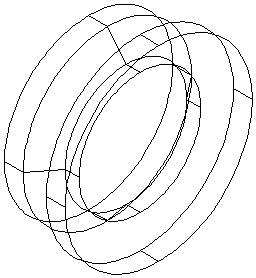
\includegraphics[width=0.4\columnwidth]{qudonghejianmo5}}
\ffigbox{\caption{构建$\phi 20$圆柱孔}\label{fig:qudonghejianmo6}}{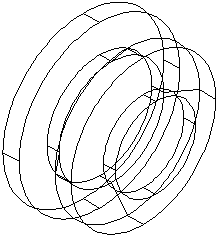
\includegraphics[width=0.4\columnwidth]{qudonghejianmo6}}
\end{floatrow}
\end{figure}

然后使用并集命令,将$\phi 40$圆柱体并入之前所构建的模型之中,构成一个整体。

\begin{lstlisting}
命令: UNION
选择对象: 找到 1 个
选择对象: 找到 1 个,总计 2 个
选择对象:
\end{lstlisting}

\item 构建$\phi 20$圆柱孔

由于$\phi 20$圆柱孔位于$\phi 36$圆柱体之上,因此先将视图方向切换至西南等轴测。

\begin{lstlisting}
命令: -VIEW
输入选项 [?/删除(D)/正交(O)/恢复(R)/保存(S)/设置(E)/窗口(W)]: swiso
\end{lstlisting}

拉下来以$\phi 36$圆柱体的前圆心为圆心构建$\phi 20$圆柱体。

\begin{lstlisting}
命令: CYLINDER
指定底面的中心点或 [三点(3P)/两点(2P)/切点、切点、半径(T)/椭圆(E)]:
指定底面半径或 [直径(D)] <20.0000>: 10
指定高度或 [两点(2P)/轴端点(A)] <4.0000>: -3
\end{lstlisting}

然后,用差集命令从$\phi 30$圆柱体中去$\phi 20$圆柱体,以构建$\phi 20$圆柱孔,结果如图\ref{fig:qudonghejianmo6}所示。

\begin{lstlisting}
命令: SUBTRACT
选择要从中减去的实体、曲面和面域...
选择对象: 找到 1 个
选择对象:  选择要减去的实体、曲面和面域...
选择对象: 找到 1 个
选择对象:
\end{lstlisting}

\item 构建$\phi 14$圆柱孔

\begin{figure}[htbp]
\centering
\begin{floatrow}[2]
\ffigbox{\caption{构建$\phi 14$圆柱体}\label{fig:qudonghejianmo7}}{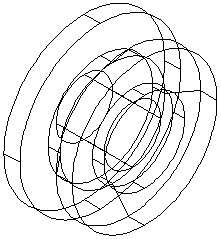
\includegraphics[width=0.4\columnwidth]{qudonghejianmo7}}
\ffigbox{\caption{构建定位槽基础实体}\label{fig:qudonghejianmo8}}{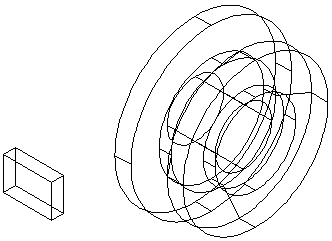
\includegraphics[width=0.6\columnwidth]{qudonghejianmo8}}
\end{floatrow}
\end{figure}

接下来,以$\phi 40$圆柱体的后圆圆心为圆心构建$\phi 14$圆柱体。
\begin{lstlisting}
命令: CYLINDER
指定底面的中心点或 [三点(3P)/两点(2P)/切点、切点、半径(T)/椭圆(E)]:
指定底面半径或 [直径(D)] <10.0000>: 7
指定高度或 [两点(2P)/轴端点(A)] <-3.0000>: 12
\end{lstlisting}

然后从复合体中去掉$\phi 14$圆柱体,形成$\phi 14$圆柱孔,结果如图\ref{fig:qudonghejianmo7}所示。
\begin{lstlisting}
命令: SUBTRACT
选择要从中减去的实体、曲面和面域...
选择对象: 找到 1 个
选择对象:  选择要减去的实体、曲面和面域...
选择对象: 找到 1 个
选择对象:
\end{lstlisting}

\item 构建定位槽

为方便准确地构建定位槽,首先在AutoCAD绘图区的任意位置绘制一个高为8.1的长方体,结果如图\ref{fig:qudonghejianmo8}所示。
\begin{lstlisting}
命令: BOX
指定第一个角点或 [中心(C)]:
指定其他角点或 [立方体(C)/长度(L)]: @3,8.1
指定高度或 [两点(2P)] <12.0000>:
\end{lstlisting}

\begin{figure}[htbp]
\centering
\subfloat[]{\label{fig:qudonghejianmo9}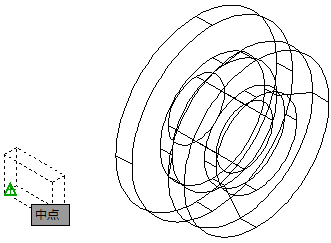
\includegraphics[width=0.35\columnwidth]{qudonghejianmo9}}\hspace{60pt}
\subfloat[]{\label{fig:qudonghejianmo10}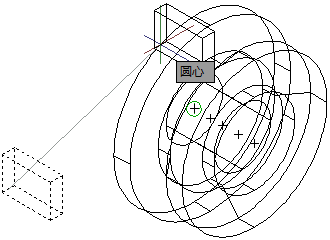
\includegraphics[width=0.35\columnwidth]{qudonghejianmo10}}
\caption{长方体移动操作}
\end{figure}

接下来,选择图\ref{fig:qudonghejianmo9}所示的长方体底边中点作为移动基点,选择图\ref{fig:qudonghejianmo10}所示$\phi 40$圆柱体后圆圆心为移动目标点,将长方体移动到$\phi 14$圆柱孔中,完成移动后结果如图\ref{fig:qudonghejianmo11}所示。
\begin{lstlisting}

命令: MOVE
选择对象: 找到 1 个
选择对象:
指定基点或 [位移(D)] <位移>:
指定第二个点或 <使用第一个点作为位移>:
\end{lstlisting}

\begin{figure}[htbp]
\centering
\subfloat[]{\label{fig:qudonghejianmo11}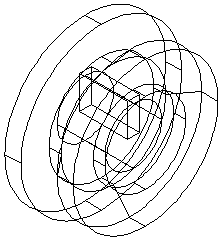
\includegraphics[width=0.3\columnwidth]{qudonghejianmo11}}\hspace{60pt}
\subfloat[]{\label{fig:qudonghejianmo12}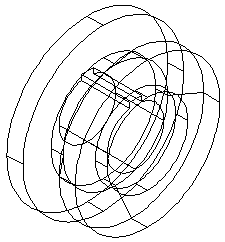
\includegraphics[width=0.3\columnwidth]{qudonghejianmo12}}
\caption{构建定位槽}
\end{figure}
 
接下来,用差集命令将长方体从复合模型中去掉,结果如图\ref{fig:qudonghejianmo12}所示。
\begin{lstlisting}
命令: SUBTRACT
选择要从中减去的实体、曲面和面域...
选择对象: 找到 1 个
选择对象:  选择要减去的实体、曲面和面域...
选择对象: 找到 1 个
选择对象:
\end{lstlisting}

\item 构建单个凸台

要构建凸台需要先构建凸台拉伸特征平面。为了方便准确地定位和构建凸台,需要先绘制一线辅助线来帮助我们准确的绘制图线。使用构造线能够方便地绘制出想要的辅助线。AutoCAD调用构建线命令的方式有:
\begin{itemize}
	\item 键盘输入xline\index{xline,构造线}
	\item 【绘图】$\rightarrow$【构造线】
	\item 【绘图】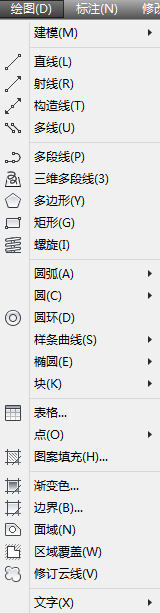
\includegraphics[scale=0.45]{drawtools}工具中的
\includegraphics[scale=0.45]{faceextude.png}图标	
\end{itemize}

首先,用构造线命令的【水平(H)】选项在绘图区绘制一条水平构造线。

\begin{lstlisting}
命令: xline
指定点或 [水平(H)/垂直(V)/角度(A)/二等分(B)/偏移(O)]: h
指定通过点:
指定通过点:
\end{lstlisting}

接下来,用构造线命令的【垂直(V)】选项在绘图区绘制一条垂直构造线。至此我们构建了两条相互垂直的辅助线,结果如图\ref{fig:qudonghejianmo13-1}所示。

\begin{figure}[htbp]
\centering
\subfloat[]{\label{fig:qudonghejianmo13-1}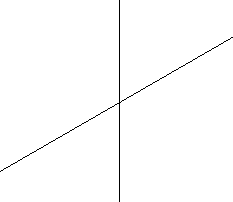
\includegraphics[width=0.3\columnwidth]{qudonghejianmo13-1}}\hspace{60pt}
\subfloat[]{\label{fig:qudonghejianmo13}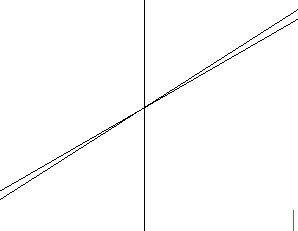
\includegraphics[width=0.3\columnwidth]{qudonghejianmo13}}
\caption{构建辅助线}
\end{figure}

\begin{lstlisting}
命令: XLINE
指定点或 [水平(H)/垂直(V)/角度(A)/二等分(B)/偏移(O)]: v
指定通过点:
指定通过点:
\end{lstlisting}

接下来,用构造线命令的【角度(A)】选项来构建角度为3度的构造线,通过点为水平构造线和垂直构造线的交点作为通过点。完成后结果如图\ref{fig:qudonghejianmo13} 所示。

\begin{lstlisting}
命令: xline
指定点或 [水平(H)/垂直(V)/角度(A)/二等分(B)/偏移(O)]: a
输入构造线的角度 (0) 或 [参照(R)]:  3
指定通过点:
指定通过点:
\end{lstlisting}

接下来,绘制另一条对称的角度构建线,AutoCAD中绘制对称图形通常采用对称镜像命令来完成,其调用方式有:
\begin{itemize}
	\item 键盘输入mirror\index{mirror,镜像}
	\item 【修改】$\rightarrow$【镜像】
	\item 【修改】
\includegraphics[scale=0.45]{edittools}工具中的【镜像】
\includegraphics[scale=0.45]{mirrortool}图标	
\end{itemize}

镜像命令调用后,选择图\ref{fig:qudonghejianmo14}所示的构造线作为镜像对象,选择图\ref{fig:qudonghejianmo15}所示的交点为镜像线的第一点,选择图\ref{fig:qudonghejianmo16}所示的位置为镜像线的第二点。最终镜像结果如图\ref{fig:qudonghejianmo17}所示。
\begin{lstlisting}
命令: mirror
选择对象: 找到 1 个
选择对象:  
指定镜像线的第一点:
指定镜像线的第二点:
要删除源对象吗?[是(Y)/否(N)] <N>:
\end{lstlisting}

\begin{figure}[htbp]
\centering
\subfloat[]{\label{fig:qudonghejianmo14}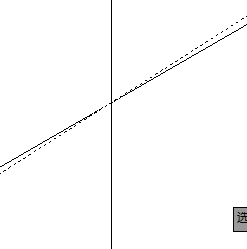
\includegraphics[width=0.2\columnwidth]{qudonghejianmo14}}\hspace{20pt}
\subfloat[]{\label{fig:qudonghejianmo15}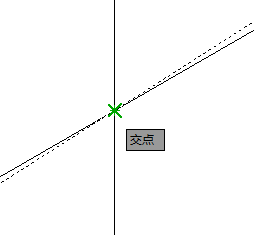
\includegraphics[width=0.2\columnwidth]{qudonghejianmo15}}\hspace{20pt}
\subfloat[]{\label{fig:qudonghejianmo16}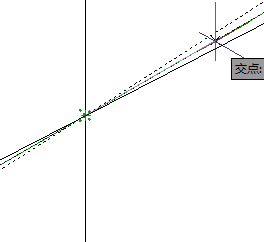
\includegraphics[width=0.2\columnwidth]{qudonghejianmo16}}\hspace{20pt}
\subfloat[]{\label{fig:qudonghejianmo17}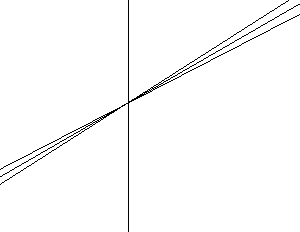
\includegraphics[width=0.2\columnwidth]{qudonghejianmo17}}
\caption{镜像操作}
\end{figure}

接下来绘制$\phi 36$的圆弧。在AutoCAD中可能用圆弧命令来完成圆弧的绘制,其调用方法有:
\begin{itemize}
	\item 键盘输入arc\index{arc,圆弧}
	\item 【绘图】$\rightarrow$【圆弧】$\rightarrow$【圆心、起点、角度】
	\item 【绘图】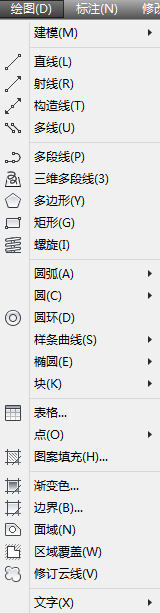
\includegraphics[scale=0.45]{drawtools}工具中的【圆弧】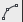
\includegraphics[scale=0.45]{arctool}图标	
\end{itemize}

由于本例中的圆弧的起点位置、圆心位置和圆弧角度都是已知的,因此圆弧命令调用后,选择【圆心(C)】选项并选择辅助线的交点作为圆。由于默认状态下,圆弧是按逆时针方向绘制的。因此用相对坐标$ @18<-3$指定圆弧的点位置,然后指定角度为6度,其最终结果如图\ref{fig:qudonghejianmo18}所示。
\begin{lstlisting}
命令: arc
指定圆弧的起点或 [圆心(C)]: c
指定圆弧的圆心:
指定圆弧的起点: @18<-3
指定圆弧的端点或 [角度(A)/弦长(L)]: a
指定包含角: 6
\end{lstlisting}


\begin{figure}[htbp]
\centering
\subfloat[]{\label{fig:qudonghejianmo18}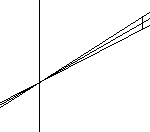
\includegraphics[width=0.3\columnwidth]{qudonghejianmo18}}\hspace{60pt}
\subfloat[]{\label{fig:qudonghejianmo19}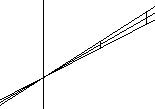
\includegraphics[width=0.3\columnwidth]{qudonghejianmo19}}
\caption{绘制圆弧}
\end{figure}

接下来,以图\ref{fig:qudonghejianmo18}中所绘的圆弧为偏移对象,得到直径$\phi 20$的圆弧,结果如图\ref{fig:qudonghejianmo19}所示。

\begin{lstlisting}
命令: offset
当前设置: 删除源=否  图层=源  OFFSETGAPTYPE=0
指定偏移距离或 [通过(T)/删除(E)/图层(L)] <通过>:  8
选择要偏移的对象,或 [退出(E)/放弃(U)] <退出>:
指定要偏移的那一侧上的点,或 [退出(E)/多个(M)/放弃(U)] <退出>:
选择要偏移的对象,或 [退出(E)/放弃(U)] <退出>:
\end{lstlisting}

接下来需要将不需要的线条删除,由于只删除同一条图线的部分,所以不能够使用删除命令。在AutoCAD中实现线段部分删除的命令是修剪,调用该命令的方式有
\begin{itemize}
	\item 键盘输入trim\index{trim,修剪}
	\item 【修改】$\rightarrow$【修剪】
	\item 【修改】
\includegraphics[scale=0.45]{edittools}工具中的【修剪】
\includegraphics[scale=0.45]{trimtool}图标	
\end{itemize}

修剪命令调用后,选择图\ref{fig:qudonghejianmo20}所示的两条圆弧为修剪边,然将图形修剪为图\ref{fig:qudonghejianmo21}所示的结果。

\begin{lstlisting}
命令: trim
视图与 UCS 不平行。命令的结果可能不明显。
当前设置:投影=UCS,边=无
选择剪切边...
选择对象或 <全部选择>:  找到 1 个
选择对象: 找到 1 个,总计 2 个
选择对象:
选择要修剪的对象,或按住 Shift 键选择要延伸的对象,或
[栏选(F)/窗交(C)/投影(P)/边(E)/删除(R)/放弃(U)]:  指定对角点:
选择要修剪的对象,或按住 Shift 键选择要延伸的对象,或
[栏选(F)/窗交(C)/投影(P)/边(E)/删除(R)/放弃(U)]:
选择要修剪的对象,或按住 Shift 键选择要延伸的对象,或
[栏选(F)/窗交(C)/投影(P)/边(E)/删除(R)/放弃(U)]:
选择要修剪的对象,或按住 Shift 键选择要延伸的对象,或
[栏选(F)/窗交(C)/投影(P)/边(E)/删除(R)/放弃(U)]:
\end{lstlisting}

\begin{figure}[htbp]
\centering
\subfloat[]{\label{fig:qudonghejianmo20}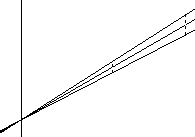
\includegraphics[width=0.3\columnwidth]{qudonghejianmo20}}\hspace{60pt}
\subfloat[]{\label{fig:qudonghejianmo21}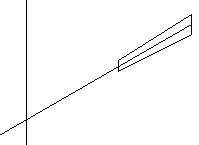
\includegraphics[width=0.3\columnwidth]{qudonghejianmo21}}
\caption{修剪操作}
\end{figure}

完成修剪后,将所得拉伸特征面进面域操作,使构成一个封闭平面。

\begin{lstlisting}
命令: region
选择对象: 指定对角点: 找到 4 个
选择对象:
已提取 1 个环。
已创建 1 个面域。
\end{lstlisting}

最后,运用AutoCAD中的实体拉伸命令将其构建为凸台。在AutoCAD中,实体拉伸命令的调用方式有:
\begin{itemize}
	\item 键盘输入extrude\index{extrude,拉伸}
	\item 【绘图】$\rightarrow$【建模】$\rightarrow$【拉伸】
	\item 【建模】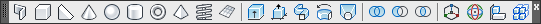
\includegraphics[scale=0.45]{solidtoolbar}工具中的【拉伸】
\includegraphics[scale=0.45]{extrudetool}图标	
\end{itemize}

调用拉伸命令后,选择图\ref{fig:qudonghejianmo23}所示的面域作为拉伸对象,并用【倾斜角(T)】选项将倾斜角指定为10度,指定拉伸高度为1mm,结果如图\ref{fig:qudonghejianmo24}所示。
\begin{lstlisting}
命令: EXTRUDE
当前线框密度:  ISOLINES=4,闭合轮廓创建模式 = 实体
选择要拉伸的对象或 [模式(MO)]: 找到 1 个
选择要拉伸的对象或 [模式(MO)]:
指定拉伸的高度或 [方向(D)/路径(P)/倾斜角(T)/表达式(E)] <12.0000>: t
指定拉伸的倾斜角度或 [表达式(E)] <0>: 10
指定拉伸的高度或 [方向(D)/路径(P)/倾斜角(T)/表达式(E)] <12.0000>: 1
\end{lstlisting}

\begin{figure}[htbp]
\centering
\subfloat[]{\label{fig:qudonghejianmo23}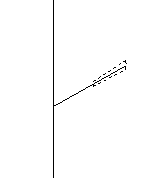
\includegraphics[width=0.3\columnwidth]{qudonghejianmo23}}\hspace{60pt}
\subfloat[]{\label{fig:qudonghejianmo24}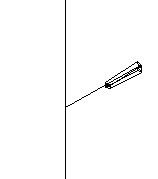
\includegraphics[width=0.3\columnwidth]{qudonghejianmo24}}
\caption{拉伸操作}
\end{figure}

\item 构建凸台阵列

由于驱动盒的凸台是呈环形分布,且数量有36个,若采用单个凸台的构建方式,不仅费时费力,还容易出错。在AutoCAD中可以用三维阵列来实现多个相同实体的构建和规律排列,其调用方式有:
\begin{itemize}
	\item 键盘输入3darray\index{3darray,三维阵列}
	\item 【修改】$\rightarrow$【三维操作】$\rightarrow$【三维阵列】
	\item 【建模】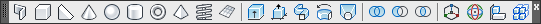
\includegraphics[scale=0.45]{solidtoolbar}工具中的【拉伸】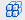
\includegraphics[scale=0.45]{3darraytool}图标	
\end{itemize}

\begin{figure}[htbp]
\centering
\subfloat[]{\label{fig:qudonghejianmo25}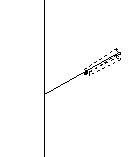
\includegraphics[width=0.2\columnwidth]{qudonghejianmo25}}\hspace{20pt}
\subfloat[]{\label{fig:qudonghejianmo26}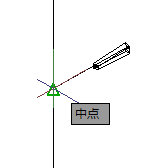
\includegraphics[width=0.2\columnwidth]{qudonghejianmo26}}\hspace{20pt}
\subfloat[]{\label{fig:qudonghejianmo27}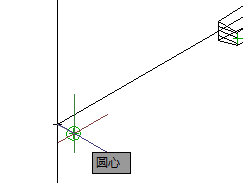
\includegraphics[width=0.2\columnwidth]{qudonghejianmo27}}\hspace{20pt}
\subfloat[]{\label{fig:qudonghejianmo28}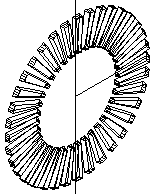
\includegraphics[width=0.2\columnwidth]{qudonghejianmo28}}
\caption{三维镜像操作}
\end{figure}

三维命令调用后,选择图\ref{fig:qudonghejianmo25}所示凸台作为阵列对象,通过【环形(P)】选项将阵列方式设置为环形,并将项目数设置为36,填空角度设置为360度,然后选择图\ref{fig:qudonghejianmo26}所示点为阵列中心,选择图\ref{fig:qudonghejianmo27}凸台的前圆心作为阵列轴上的第二点。三阵列完成后的结果如图\ref{fig:qudonghejianmo28}所示。
\begin{lstlisting}
命令: 3darray
正在初始化...  已加载 3DARRAY。
选择对象: 找到 1 个
选择对象:
输入阵列类型 [矩形(R)/环形(P)] <矩形>:p
输入阵列中的项目数目: 36
指定要填充的角度 (+=逆时针, -=顺时针) <360>:
旋转阵列对象? [是(Y)/否(N)] <Y>:
指定阵列的中心点:
指定 UCS 的原点或 [面(F)/命名(NA)/对象(OB)/上一个(P)/视图(V)/世界(W)/X/Y/Z/Z 轴(ZA)] <世界>: _ZAXIS
指定新原点或 [对象(O)] <0,0,0>:
在正 Z 轴范围上指定点 <-266.1915,360.4101,1.0000>:
\end{lstlisting}

\item 组合构建驱动盒模型

至此,在绘图区中已经完成了驱动盒两个组成部分的构建。接下来需要用移动命令将其中一部分移动到准确的组合点上,以便进行组合。根据移少不移多的原则,因此选择$\phi 36$圆柱体的前圆心作为移动基点,将其移动到辅助线的交叉点上,结果如图\ref{fig:qudonghejianmo29}所示。

\begin{figure}[htbp]
\centering
\begin{floatrow}[2]
\ffigbox{\caption{移动结果}\label{fig:qudonghejianmo29}}{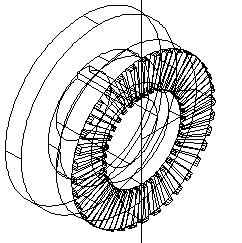
\includegraphics[width=0.4\columnwidth]{qudonghejianmo29}}
\ffigbox{\caption{驱动盒三维模型}\label{fig:qudonghejianmo30}}{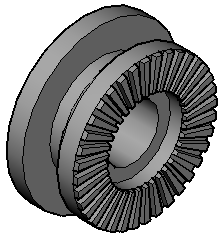
\includegraphics[width=0.4\columnwidth]{qudonghejianmo30}}
\end{floatrow}
\end{figure}
\begin{lstlisting}
命令: move
选择对象: 找到 1 个
选择对象:
指定基点或 [位移(D)] <位移>:
指定第二个点或 <使用第一个点作为位移>:
\end{lstlisting}

完成移动后,将所有的实体合并成为一个整体,构成驱动盒的三维模型。
\begin{lstlisting}
命令: UNION
选择对象: 指定对角点: 找到 38 个
选择对象:
\end{lstlisting}

合并完成后需要将多余的辅助线删除,只保留驱动盒的三维模型。

\begin{lstlisting}
命令: erase
选择对象: 找到 1 个
选择对象: 找到 2个
选择对象:
\end{lstlisting}

\item 切换视觉样式

为方便观察驱动盒的三维模型,我们将视觉样式切换为灰度,结果如图\ref{fig:qudonghejianmo30}所示。
\begin{lstlisting}
命令: VSCURRENT
输入选项 [二维线框(2)/线框(W)/隐藏(H)/真实(R)/概念(C)/着色(S)/带边缘着色(E)/灰度(G)/勾画(SK)/X 射线(X)/其他(O)] <二维线框>: g
\end{lstlisting}

\item 保存模型

最后将驱动盒三维模型保存为“驱动盒.dwg”。
\end{procedure}